\documentclass[8pt]{mpscheatsheet}
\usepackage{amsmath, amssymb, mathtools, mathabx}
\usepackage[thinlines]{easytable}
\author{Micha Bosshart - bmicha@ethz.ch}
\title{Theory of Robotics and Mechatronics}

\newcommand{\matlab}[1]{%
    {\fontfamily{qcr}\selectfont #1}%
}

\begin{document}
    \section{Mechanical Design}
        \subsection{DOF \& DOM \& DOF EE}
    \begin{description}
        \item[DOF:] Indep. of Robot Configuration (2D: 3, 3D: 6)
        \item[DOM:] \# Joints
        \item[DOF EE:] Indep. Instant. Motions of End-Effector
    \end{description}
    \subsubsubsection{Grübler's Formula}
        \vspace{0.5em}
        $$
            DOF = C (N-g) + \sum_{i=1}^g f_i
        $$
        \begin{minipage}{0.55\linewidth}
            \begin{description}
                \item[$C$]\,: 3(2D), 6(3D)
                \item[$N$]: \# links w/out baselinks
            \end{description}
        \end{minipage}
        \begin{minipage}{0.44\linewidth}
            \begin{description}
                \item[$f_i$]: \# DOF of $i^{th}$ joint 
                \item[$g$]\,\,: \# joints   
            \end{description}
        \end{minipage}
\subsection{Precision and Accuracy}
    Need more than one measurement to be determined.
    % \vspace{-1em}
    \begin{center}
    	\resizebox{\linewidth}{!}{
    		\includegraphics[
    			page = {3},
    			% trim = {5.8cm, 1.6cm, 5.7cm, 6.75cm}, % with blue frame
    			trim = {6.2cm, 2cm, 6.1cm, 7.15cm}, %left bottom right top
    			clip
    		]{Mechanical_Design/01_2020-09-29_Mechanical-Design.pdf}
    	}
    \end{center}
    \begin{description}
        \item[Precision] "Repeatability" of two+ measurements; $\textrm{std}(M)$ 
        \item[Accuracy] "Closeness" to a standard or known value Accuracy mean; $\textrm{mean}(M) - M_R$
    \end{description}
\subsection{Resolution}
    \textbf{Actuator:} Smallest commendable distance\\
    \textbf{Sensor:} Smallest measurable interval  
    \section{Spatial Description}   
        \vspace{-0.5em}
$$
    P^0 = R_1^0 P^1 + T_1^0
$$
\subsection{Rotations}
    \subsubsection{Rotational Matrix \texorpdfstring{\hfill $R_{x_{i,\theta}}$}{}}
        \vspace{-1em}
        % $$
        % s_\theta \vcentcolon= \sin(\theta) \qquad c_\theta \vcentcolon= \cos(\theta)
        % $$
        $$
        \begin{bmatrix}
            1 & 0 & 0\\
            0 & c_\theta &-s_\theta\\
            0 & s_\theta & c_\theta
        \end{bmatrix}_x
        \quad
        \begin{bmatrix}
            c_\theta &0 & s_\theta\\
            0 & 1 & 0\\
            -s_\theta & 0 & c_\theta
        \end{bmatrix}_y
        \quad
        \begin{bmatrix}
            c_\theta &-s_\theta& 0\\
            s_\theta & c_\theta& 0\\
            0 & 0 & 1
        \end{bmatrix}_z
        $$
        $$
            R^{-1} = R^T \qquad \det(R) = \pm 1
        $$
        %  \subsubsubsection{Properties}
        %     \begin{itemize}
        %         \item orthogonal
        %         \item $R^{-1} = R^T$
        %         \item $\det(R) = \pm 1$
        %     \end{itemize}
    \subsubsection{Composition of Rotations}
        \subsubsubsection{Post Multiply}
            About "new"/ current frame of object:
            \begin{center}
                \resizebox{\linewidth}{!}{
                    \includegraphics[
                        page = {3},
                        trim = {4.9cm, 8.8cm, 5.2cm, 4.7cm}, %left bottom right top
                        clip
                    ]{Spatial_Description/01_2020-09-29_Spatial-Description.pdf}
                }
            \end{center}
        \subsubsubsection{Pre Multiply \hfill "Fixed First"}
            About original/ fixed frame:
            \begin{center}
                \resizebox{\linewidth}{!}{
                    \includegraphics[
                        page = {3},
                        trim = {4.9cm, 2.3cm, 5.2cm, 11.7cm}, %left bottom right top
                        clip
                    ]{Spatial_Description/01_2020-09-29_Spatial-Description.pdf}
                }
            \end{center}
    \subsection{Homogeneous Transformation}
        \subsubsubsection{Principle}
            \vspace{0.5em}
            $$
                y = ax + b, \qquad y = \begin{bmatrix}a&b\end{bmatrix}\begin{bmatrix}x\\1\end{bmatrix}, \qquad \begin{bmatrix}y\\1\end{bmatrix} = \begin{bmatrix}a&b\\0&1\end{bmatrix}\begin{bmatrix}x\\1\end{bmatrix}
            $$
        \subsubsubsection{Application \hfill $H_1^0$}
            \vspace{0.5em}
            $$
                P^0 = R_1^0 P^1 + T_1^0 \quad\longrightarrow\quad P_H^0 = H_1^0 P_H^1
            $$
            $$
               \begin{bmatrix} P^0\\1 \end{bmatrix} = \underbrace{\begin{bmatrix} R_1^0 & T_1^0\\ [0] &1 \end{bmatrix}}_{H_1^0} \begin{bmatrix} P^1\\1 \end{bmatrix}
            $$
            {\small $T_1^0$: Translation from 0 to 1}
        \subsubsubsection{Inverse \hfill $\left(H_1^0\right)^{-1}$}
            \vspace{0.5em}
            $$
                \left(H_1^0\right)^{-1} = H_0^1 = \begin{bmatrix}
                    \left(R_1^0\right)^T & -\left(R_1^0\right)^T T_1^0\\[.5em]
                    [0] & 1
                \end{bmatrix}
            $$
            

        
    \section{Screw Theory}
        %!Tex root=ZF_bmicha_TRM.tex
\subsection{Rigid Body Transformation}
    A mapping $g$ is a rigid body transformation if:
    \begin{itemize}
        \item \textbf{length} (distances between pts.) is preserved
            $$
                \lVert g(q) - g (p) \rVert = \lVert q - p \rVert
            $$
        \item \textbf{crossproduct} (orientation) is preserved:
            $$
                g(v\times w) = g(v) \times g(w)
            $$
    \end{itemize}
\subsection{Mathematical Remarks}
    \subsubsection{Skew - Symmetric Matrix \texorpdfstring{\hfill $\widehat{a}$}{}}
        \vspace{-1em}
        $$
            a \times b = \widehat{a} b = 
            \begin{bmatrix}
                0   & -a_3 &  a_2\\
                a_3 &    0 & -a_1\\
                -a_2&  a_1 &    0
            \end{bmatrix}
            b
            =
            \begin{bmatrix}
                a_2 b_3 - a_3 b_2\\
                a_3 b_1 - a_1 b_3\\
                a_1 b_2 - a_2 b_1
            \end{bmatrix}
        $$
    \subsubsection{Matrix Exponential}
        \vspace{-0.5em}
        \begin{align*}
            e^{\widehat{\omega} \theta} &= \mathbb{I} + \widehat{\omega} \theta + \frac{1}{2!} (\widehat{\omega} \theta)^2 + \frac{1}{3!} (\widehat{\omega} \theta)^3 + \dots\\[0.5em]
                                        &\overset{*}{=} \mathbb{I} + \widehat{\omega} \sin\theta + \widehat{\omega}^2 (1 -\cos\theta)
        \end{align*}
        $(*)$ Rodrigues' Formula
\subsection{Screw Parameters \& Twist}
        All parameters respresented in \textbf{reference frame}.
    \begin{description}
        \item[Pitch $h$]: Ratio of translational and rotational motion
        \item[Axis $l$]: Axis of rotation / direction of translation
        \item[Magnitude $M$]: Amount of rotation/ translation  
        % \item[Twist $\widehat{\xi}$]
        % \item[Twist Coordinates $\xi$] 
    \end{description}

    \subsubsubsection{General Case}
        \begin{align*}
            h = \frac{\omega^T v}{\lVert \omega^2 \rVert} && l = \frac{\omega \times v}{\lVert \omega^2 \rVert} + \lambda \omega && M = \lVert \omega \rVert
        \end{align*}
        \begin{align*}
            \widehat{\xi} &= 
                \begin{bmatrix}
                    &\widehat{\omega} & & - \omega \times q + h \omega\\
                    0 & 0 & 0 & 0 \\
                \end{bmatrix}
            &\in \mathbb{R}^{4 \times 4}\\
            \xi &= 
                \begin{bmatrix}
                    - \omega \times q + h \omega\\
                    \omega
                \end{bmatrix}
            &\in \mathbb{R}^{6 \times 1}
        \end{align*}
    \subsubsubsection{Rotation}
        \begin{align*}
            h = 0 && l = q + \lambda \omega && M = \theta
        \end{align*}
        \begin{align*}
            \widehat{\xi} &= 
                \begin{bmatrix}
                    &\widehat{\omega} & & - \omega \times q\\
                    0 & 0 & 0 & 0 \\
                \end{bmatrix}
            \\
            \xi &= 
                \begin{bmatrix}
                    - \omega \times q\\
                    \omega
                \end{bmatrix}
        \end{align*}
    \subsubsubsection{Translation}
        \begin{align*}
            h = \infty && l = \lambda v && M = \theta
        \end{align*}
        \begin{align*}
            \widehat{\xi} &= 
                \begin{bmatrix}
                    0 & v\\
                    0 & 0 \\
                \end{bmatrix} \in \mathbb{R}^{4 \times 4}
            \\
            \xi &= 
                \begin{bmatrix}
                   v\\
                   0    
                \end{bmatrix} \in \mathbb{R}^{6 \times 1}
        \end{align*}
    \subsection{Matrix Exponentials}
        \vspace{-1em}
        $$\boxed{%
            g_{st}(\theta_1,\dots ,\theta_n) = e^{\widehat{\xi}_1 \theta_1} \cdots e^{\widehat{\xi}_n \theta_n} \cdot g_{st}(0) = H_n^0
        }$$
        $g_{st}(0)$: IC of $n^{th}$ frame w.r.t. $0^{th}$ frame.
    \subsubsection{Homogeneous Transformation}
    The twist matrix exponential yields a Homogeneous Transformation. For $\lVert \omega \rVert = \lVert v \rVert = 1$
    $$
        e^{\widehat{\xi} \theta} =
        \begin{bmatrix}
            e^{\widehat{\omega} \theta} & \left( \mathbb{I} - e^{\widehat{\omega} \theta} \right) ( \omega \times v) + h \theta \omega\\
            0 & 1
        \end{bmatrix} \in \mathbb{R}^{4 \times 4}
    $$
    \vskip0.5em
    \begin{minipage}{0.49\linewidth}
        \begin{center}
            \textbf{Revolute}
        \end{center}
        $$
            \begin{bmatrix}
                e^{\widehat{\omega} \theta} & \left( \mathbb{I} - e^{\widehat{\omega} \theta} \right) ( \omega \times v)\\
                0 & 1
            \end{bmatrix}
        $$
    \end{minipage}
    \begin{minipage}{0.49\linewidth}
        \begin{center}
            \textbf{Prismatic}
        \end{center}
        $$
            \begin{bmatrix}
                \mathbb{I} & \theta v\\
                0 & 1
            \end{bmatrix}
        $$
    \end{minipage}
    \subsubsection{Initial Coniditions}
        \vspace{-1em}
        $$\boxed{%
            g_{ab}(\theta) = e^{\widehat{\xi} \theta} \cdot g_{ab}(0)
        }$$
        \textbf{$g_{ab}(0)$} describes transformation from base to toolframe.
        $$
            g_{ab}(0) = \begin{bmatrix}
                R(0) & q\\
                0 & 1
            \end{bmatrix}
        $$  
\subsection{Matlab - Kinematics Toolbox}
    \begin{center}
        \resizebox{0.78\linewidth}{!}{
        % \resizebox{0.94\linewidth}{!}{
                \includegraphics[
                    page = {11},
                    % trim = {2.5cm, 1.6cm, 2.9cm, 2.5cm}, % with blue frame
                    trim = {2.9cm, 2cm, 3.4cm, 2.9cm}, %left bottom right top
                    clip
                ]{Screw_Theory/02_2020-10-06_ScrewTheory.pdf}
            } 
    \end{center}
    
    \section{Forward Kinematics (FK)}
        %!Tex root=ZF_bmicha_TRM.tex
\subsection{Denavit-Hartenberg (DH) Convention}
    \vspace{0.5em}
    \begin{center}
        \fbox{%
            \parbox{0.95\linewidth}{%
                The $x_i$ axis must be \textbf{perpendicular} and \textbf{intersect} the $z_{i-1}$ axis.
            }
        }
    \end{center}

    \begin{minipage}{0.54\linewidth}
        \begin{center}
            \resizebox{\linewidth}{!}{
                    \includegraphics[
                        page = {8},
                        trim = {16cm, 7cm, 7cm, 4cm}, %left bottom right top
                        clip
                    ]{Forward_Kinematics/03_2020-10-13_ForwardKinematics.pdf}
                }
        \end{center}
    \end{minipage}
    \begin{minipage}{0.45\linewidth}
        \small
        \begin{description}
            \item[\boldmath{$\theta$}:] \textbf{joint angle}\\ (about original z-axis) 
            \item[\boldmath{$d$}:]      \textbf{link offset}\\ (along original z-axis) 
            \item[\boldmath{$a$}:]      \textbf{link length}\\ (along current x-axis) 
            \item[\boldmath{$\alpha$}:] \textbf{link twist} \\ (about current x-axis) 
        \end{description}
    \end{minipage}
    \subsubsubsection{Example}
    \vspace{0.5em}
    \begin{minipage}{0.5\linewidth}
        \begin{center}
            \resizebox{\linewidth}{!}{
                    \includegraphics[
                        page = {9},
                        trim = {2.5cm, 1.5cm, 20.5cm, 4cm}, %left bottom right top
                        clip
                    ]{Forward_Kinematics/03_2020-10-13_ForwardKinematics.pdf}
                }
        \end{center}
    \end{minipage}
    \hfill
    \begin{minipage}{0.39\linewidth}
        \begin{center}
            \resizebox{\linewidth}{!}{
                    \includegraphics[
                        page = {9},
                        trim = {16.7cm, 6.3cm, 8.42cm, 8.7cm}, %left bottom right top
                        clip
                    ]{Forward_Kinematics/03_2020-10-13_ForwardKinematics.pdf}
                }
        \end{center}
    \end{minipage}
    
    
    
    \subsubsubsection{Homogeneous Transformation}
        \begin{center}
            All operations w.r.t. \textbf{current frame!}
        \end{center}
        $$\boxed{
            A_i = \textrm{Rot}_z(\theta)\ \textrm{Trans}_z(d)\ \textrm{Trans}_x(a)\ \textrm{Rot}_x(\alpha) = H_i^{i-1}
        }$$
        {\scriptsize
        $$
            =
            \begin{bmatrix}
                c_\theta & -s_\theta & 0 & 0\\
                s_\theta & c_\theta & 0 & 0\\
                0 & 0 & 1 & 0\\
                0 & 0 & 0 & 1\\
            \end{bmatrix}\!\!
            \begin{bmatrix}
                1 & 0 & 0 & 0\\
                0 & 1 & 0 & 0\\
                0 & 0 & 1 & d\\
                0 & 0 & 0 & 1\\
            \end{bmatrix}\!\!
            \begin{bmatrix}
                1 & 0 & 0 & a\\
                0 & 1 & 0 & 0\\
                0 & 0 & 1 & 0\\
                0 & 0 & 0 & 1\\
            \end{bmatrix}\!\!
            \begin{bmatrix}
                1 & 0 & 0 & 0\\
                0 & c_\alpha & -s_\alpha & 0\\
                0 & s_\alpha & c_\alpha & 0\\
                0 & 0 & 0 & 1\\
            \end{bmatrix}
        $$
        $$
            = 
            \begin{bmatrix}
                c_\theta & -s_\theta c_\alpha &  s_\theta s_\alpha & a c_\theta\\
                s_\theta &  c_\theta c_\alpha & -c_\theta c_\alpha & a s_\theta\\
                0        &  s_\alpha          &  c_\alpha          & d\\
                0        &  0                 &  0                 & 1
            \end{bmatrix}
        $$}
    \subsubsubsection{Choosing Axis}
            \begin{enumerate}
                \item Set z axis along rotational or translational axis
                \item Set x axis according to DH convention
                \item Set y axis using right hand rule
            \end{enumerate}
        
\subsection{Definitions}
    \subsubsection{Workspaces}
        \textbf{Reachable Workspace:} EE Origin can reach with at least 1 orientation\\
        \textbf{Dexterous Workspace:} EE Origin can reach with multiple orientations
    \subsubsection{Joint- \& Taskspace}
        \textbf{Jointspace:} Independent, actuated parameters\\
        \textbf{Taskspace:} Position \& orientation of EE

    \vfill \null \columnbreak
    \section{Rigid Body Velocity}
        %!Tex root=ZF_bmicha_TRM.tex
\subsection{Angular Velocity}
    \vspace{-1em}
    \begin{align*}
        q_a(t) = R_{ab}(t) \cdot q_b && v_{q_a}(t) = \dot{R}_{ab}(t) \cdot q_b
    \end{align*}
    \vspace{0em}
    \begin{center}
        \begin{tabular}{cp{2em}c}
            \textbf{Spatial Angular Vel.} && \textbf{Body Angular Vel.}\\[0.5em]
            $\widehat{\omega}_{ab}^s = \dot{R}_{ab} \cdot R_{ab}^{-1}$&&$\widehat{\omega}_{ab}^b = R_{ab}^{-1} \cdot \dot{R}_{ab}$
        \end{tabular}
    \end{center}
    \begin{center}
        \begin{tabular}{c}
            \textbf{Transformation}\\[0.5em]
            $\widehat{\omega}_{ab}^b = R_{ab}^{-1} \cdot \widehat{\omega}_{ab}^s \cdot R_{ab}$
        \end{tabular}
    \end{center}
    \vspace{-4pt}
\subsection{Velocity}
    \vspace{0.5em}
    \begin{center}
        \begin{tabular}{cp{2em}c}
            \textbf{Spatial Vel.} && \textbf{Body Vel.}\\[0.5em]
            $v_{q_a} = \widehat{\omega}_{ab}^s \times q_a + v_{ab}^s$ && $v_{q_b} = \widehat{\omega}_{ab}^b \times q_b + v_{ab}^b$
        \end{tabular}
    \end{center}
    \begin{minipage}{0.495\linewidth}
        \footnotesize
        \begin{description}
            \item[$\boldsymbol{\widehat{\omega}_{ab}^s}$] is the instantaneous angular velocity of the body as viewed in the spatial frame.
            \item[$\boldsymbol{v_{ab}^{s\phantom{b}}}$] is the velocity of a point attached to the body frame and passing through the origin of the spatial frame, written in spatial coordinates.
        \end{description}        
    \end{minipage}
    \begin{minipage}{0.48\linewidth}
        \footnotesize
        \begin{description}
            \item[$\boldsymbol{\widehat{\omega}_{ab}^b}$] is the angular velocity of the body frame, written in the body coordinates.
            \item[$\boldsymbol{v_{ab}^b}$] is the velocity of the origin of the body frame (relative to the spatial frame) written in the body coordinates.
        \end{description}        
    \end{minipage}
\subsection{Twist Velocities}
        \subsubsubsection{Homogeneous Transformation \hfill $g_{ab}(t)$}
            \vspace{0.5em}
            $$
                g_{ab}(t) = 
                    \begin{bmatrix}
                        R_{ab}(t) & p_{ab}(t)\\
                        0 & 1
                    \end{bmatrix}
                    = e^{\widehat{\xi} \theta} \cdot g(0)
            $$
            \begin{align*}
                \boldsymbol{\dot{g}} &= 
                    \begin{bmatrix}
                        \dot{R} & \dot{p}\\
                        0 & 0
                    \end{bmatrix}
                &&&
                \boldsymbol{g^{-1}} &= 
                    \begin{bmatrix}
                        R^T & -R^Tp\\
                        0 & 1
                    \end{bmatrix}
                \\
                & = \widehat{\xi} \dot{\theta} \cdot e^{\widehat{\xi} \theta} \cdot g(0)
                &&&
                &= g(0)^{-1} \cdot e^{-\widehat{\xi} \theta}
                \\
                & = \widehat{\xi} \dot{\theta} \cdot g(t)
            \end{align*}
            $$
                \boldsymbol{\dot{R}} = \widehat{\omega} \cdot R
            $$
            \vspace{-0.5em}
        \subsubsubsection{Spatial Velocity}
            \textbf{Twist Form:}
            $$
                \widehat{V}_{ab}^s = \dot{g}_{ab}^{\phantom{-l}}\! \cdot g_{ab}^{-1} = 
                    \begin{bmatrix}
                        \dot{R} R^T & - \dot{R} R^T p + \dot{p}\\
                        0 & 0
                    \end{bmatrix}
                    =
                    \widehat{\xi} \dot{\theta}
            $$
            \textbf{Twist Coordinates:}
            $$  
                V_{ab}^s = 
                    \begin{bmatrix}
                        v_{ab}^s \\[0.25em] \omega_{ab}^s
                    \end{bmatrix}
                    =
                    \begin{bmatrix}
                        -\dot{R} R^T p + \dot{p}\\[0.25em] \left( \dot{R} R^T \right) \widecheck{}
                    \end{bmatrix}
                    =
                    \xi \dot{\theta}
            $$
        \subsubsubsection{Body Velocity}
            \textbf{Twist Form:}
            $$
                \widehat{V}_{ab}^b = g_{ab}^{-1} \cdot \dot{g}_{ab}^{\phantom{-1}} = 
                    \begin{bmatrix}
                        R^T \dot{R} & R^T \dot{p}\\
                        0 & 0
                    \end{bmatrix}
                    =
                    g^{-1} \widehat{V}^s g
            $$
            \textbf{Twist Coordinates:}
            $$  
                V_{ab}^b = 
                    \begin{bmatrix}
                        v_{ab}^b \\[0.5em] \omega_{ab}^b
                    \end{bmatrix}
                    =
                    \begin{bmatrix}
                        R^T \dot{p}\\[0.25em] \left( R^T \dot{R} \right) \widecheck{}
                    \end{bmatrix}
            $$
    \vfill \null \columnbreak
    \subsubsection{Transformations}
        \vspace{-1em}
        $$\boxed{%
            V_{ab}^s = \textrm{Adj}_g \cdot V_{ab}^b
        }$$
        \begin{align*}
            V_{ac}^s &= V_{ab}^s + \textrm{Adj}_{g_{ab}} \cdot V_{bc}^s\\
            V_{ac}^b &=  V_{bc}^b + \textrm{Adj}_{g_{bc}^{-1}} \cdot V_{ab}^b
        \end{align*}
    \subsubsection{Adjoint \texorpdfstring{\hfill Adj}{}}
        \vspace{-0.5em}
        \begin{align*}
            \textrm{Adj}_g &=
                \begin{bmatrix}
                    R & \widehat{p}R\\
                    0^{3 \times 3} & R
                \end{bmatrix} \in \mathbb{R}^{6 \times 6}
            \\[0.25em]
            \textrm{Adj}_g^{-1} &=
                \begin{bmatrix}
                    R^T & -R^T \widehat{p}\\
                    0^{3 \times 3} & R^T
                \end{bmatrix}
                =
                \textrm{Adj}_{g^{-1}}
        \end{align*}
    \section{Jacobian}
        %!TEX root=ZF_bmicha_TRM.tex
\vspace{-0.5em}
$$
    \begin{bmatrix}
        v_0 \\ \omega_0
    \end{bmatrix}
    = 
    \begin{bmatrix}
        J_v \\ J_\omega
    \end{bmatrix}
    \cdot 
    \begin{bmatrix}
        \dot{\theta}_1 \\ \vdots \\ \dot{\theta}_N
    \end{bmatrix}
    % ,
    % \qquad
    % \begin{bmatrix}
    %     \dot{X} \\ \dot{Y}
    % \end{bmatrix}_{\textrm{Tip}}
    % = J \cdot
    % \begin{bmatrix}
    %     \dot{\theta}_1 \\ \dot{\theta}_2
    % \end{bmatrix}
$$
        \subsection{DH-Convention}
    \vspace{-0.5em}
    $$\boxed{
        J = \begin{bmatrix}
            J_1, J_2, \dots , J_n
        \end{bmatrix} \in \mathbb{R}^{6 \times n}
    }$$
    $$
        H_i^0 = A_1 A_2 \cdots A_n = 
        \begin{bmatrix}
            X_i^0 & Y_i^0 & Z_i^0 & T_i^0\\
            0 & 0 & 0 & 1
        \end{bmatrix}
        \in \mathbb{R}^{4 \times 4}
    $$
    \begin{minipage}{0.55\linewidth}
        \begin{center}
            \hspace{8mm}\textbf{Revolute}
        \end{center}
        $$
            J_i = 
            \begin{bmatrix}
                Z_{i-1}^0 \times \left( T_n^0 - T_{i-1}^0 \right) \\[1em]
                Z_{i-1}^0
            \end{bmatrix}
        $$
    \end{minipage}
    \begin{minipage}{0.44\linewidth}
        \begin{center}
            \hspace{7mm}\textbf{Prismatic}
        \end{center}
        $$
            J_i = 
            \begin{bmatrix}
                Z_{i-1}^0 \\[1em]
                0^{3 \times 1}
            \end{bmatrix}
        $$
    \end{minipage}
        \subsection{Manipulator Jacobian}
    \vspace{-1em}
    \begin{align*}
        V_{st}^s &= J_{st}^s(\theta) \cdot \dot{\theta}\\
        V_{st}^b &= J_{st}^b(\theta) \cdot \dot{\theta}\\[1em]
        J_{st}^s(\theta) &= \textrm{Adj}_{g_{st}(\theta)} \cdot  J_{st}^b(\theta)
    \end{align*}
    \vspace{-0.5em}
    \subsubsubsection{Spatial Frame}
        \begin{align*}
            J_{st}^s(\theta) &=
                \begin{bmatrix}
                    \xi_1 & \xi_2' & \cdots & \xi_n'
                \end{bmatrix}
            \\[0.5em]
            \xi_i' &= \textrm{Adj}_{\left(e^{\widehat{\xi}_1\theta_1} \cdots\, e^{\widehat{\xi}_{i-1}\theta_{i-1}}\right)} \cdot \xi_i = \textrm{Adj}_{(g_{i-1})} \cdot \xi_i\\
            \widehat{\xi}_i' &= g_{i-1} \cdot \widehat{\xi}_i \cdot g_{i-1}^{-1}
        \end{align*}
    \subsubsubsection{Body Frame}
        \begin{align*}
            J_{st}^b(\theta) &=
                \begin{bmatrix}
                    \xi_1^+ & \xi_2^+ & \cdots & \xi_n^+
                \end{bmatrix}
            \\[0.5em]
            \xi_i^+ &= \textrm{Adj}^{-1}_{\left(e^{\widehat{\xi}_i \theta_i} \cdots\, e^{\widehat{\xi}_{n}\theta_{n}} \cdot g_{st}(0)\right)} \cdot \xi_i
        \end{align*}
        \vfill \null \columnbreak
    \subsubsection{Singularities \texorpdfstring{\hfill $\textrm{det}(J_{st}) = 0$}{\textit{Jacobian is not invertible}}}
        \textbf{Find Singularities} with $\textrm{det}(J_{st}) = 0$.\\[0.5em]
        \matlab{sings = solve(detJ==0,[th1, th2, th3]);}\vspace{0.5em}
        \textbf{Linearly Dependent Joints} have nonzero entries in ker(J).\\[0.5em]
        \matlab{th1 = singularity.th1(3);\\%
                th2 = singularity.th2(3);\\%
                th3 = singularity.th3(3);\\%
                JSingular = subs(Jnum); \% substitute syms\\%
                nullspace = null(JSingular)%
                }\vspace{0.25em}
    \subsubsection{Velocities / SVD}
        $$
            J = U \cdot \Sigma \cdot V^T 
            \qquad
            \begin{bmatrix}
                v^0 \\ \omega^0
            \end{bmatrix}
            =
            J \cdot \dot{\theta}                
        $$
        \begin{description}
            \item[Singular Values] of Jacobian correspond to amplification of joint velocities to workspace velocities.
            \item[Input Directions] correspond to \textbf{rows of $V^T$}
            \item[Output Directions] correspond to \textbf{columns of $U$}
        \end{description}
        \subsection{Inverse Kinematics}
    \vspace{-0.5em}
    $$
        \dot{\theta} = J^{-1} \cdot 
            \begin{bmatrix}
                v^0 \\ \omega^0
            \end{bmatrix}
    $$
        \subsection{Manipulability \texorpdfstring{\hfill $\mu$}{mu}}
    Closeness to singularity.
    $$
        \mu = \prod_i \sigma_i
    $$
    \begin{description}
        \item[$\sigma :$] Singular values of manipulator Jacobian. 
    \end{description}
    \section{Parallel and Redundant Robots}
        %!Tex root=ZF_bmicha_TRM.tex
\subsection{Parallel Robot}
    Two or more chains connect EE to base.
    \begin{minipage}{0.2\linewidth}
        \resizebox{\linewidth}{!}{
                \includegraphics[
                    page = {3},
                    trim = {24cm, 4cm, 2.6cm, 10.1cm}, %lbrt
                    clip
                ]{Parallel-Redundant_Robots/06_2020-11-03_Para_Red_Robots_and_InvKinematics.pdf}
            }
    \end{minipage}
\subsection{Redundant Robot}
    Has more DOFs than required to reach certain pos.\\
    \textbf{Self Motion Manifold}\\
    EE fixed $\to$ robot can still move
    \section{Force Control}
        %!Tex root=ZF_bmicha_TRM.tex
\vspace{-0.5em}
$$
    \tau = J^T \cdot F, \qquad F = [F_x, F_y, F_z, \tau_x, \tau_y, \tau_z]^T
$$
\begin{description}
    \item[$F :$] Force at EE 
    \item[$\tau :$] Joint Torque 
\end{description}

\subsection{Stiffness k}
    \vspace{-1em}
    $$
        F = k \cdot \Delta x
    $$
\subsection{Compliance}
        \subsubsubsection{Passive Compliance}
            Non-actuated tendency of a body, displaced due to external forces. (Spring)
        \subsubsubsection{Active Compliance}
            Controlled compliance in response to an external force.
    \subsubsection{Compliance Frame}
        Allows task-decomposition into pure position or force commands.
        \begin{center}
            \resizebox{0.7\linewidth}{!}{
                \includegraphics[
                    page = {12},
                    trim = {2.5cm, 7cm, 15.5cm, 4cm},
                    clip
                ]{Force_Control/10-1-Force-Control-and-Haptics.pdf}
            }
        \end{center}
        \begin{description}
            \item[Natural Constraints:] imposed by environment
                \begin{description}
                    \item[$\to$]  $f_z=0$ env won't exceed force on robot in z dir
                \end{description}
            \item[Artificial Constraints:] how we want robot to act  
                \begin{description}
                    \item[$\to$]  $f_x=0$ don't want to exceed force in x dir on env
                \end{description}
        \end{description}
        \vspace{1em}
        \begin{itemize}
            \item \# constrains = \# DOF of task space (usually 6)
            \item constraints usually come in pairs (nat \& art)
        \end{itemize}
           
\subsection{Control}
    \begin{description}
        \item[Compliance Control] Measure actual force; adjust in order to fulfill compliance constraints
        \item[Impedance Control] Similar to compliance control. System is made to behave like mass-spring-damper sys. 
        \item[Hybrid Position-Force Control] Apply position or force control along different DOFs of compliance frame.
    \end{description}
    \section{Computer Vision}
        \subsection{Thresholding / Binarization}
    Pixels with intensity \textit{below} threshold $\rightarrow$ black\\
    Pixels with intensity \textit{above} threshold $\rightarrow$ white\\
    \textbf{Threshold} usually between fore- and background peak.
    
    \subsubsection{Adaptive Thresholding}
        Compute threshold seperately for smaller regions.\\
        (useful if multiple objects present)  

    \subsubsection{Dilation/ Erosion}
        After Thresholding, regions can be distorted by noise and texture.
        \begin{description}
            \item[Dilation:] Bright regions grow
            \item[Erosion:] Bright regions shrink
        \end{description}
        \begin{center}
            \resizebox{\linewidth}{!}{
               \includegraphics[
                    page = {5},
                    trim = {5.8cm, 2.2cm, 5.8cm, 11.3cm},
                    clip
                ]{Computer_Vision/08_2020-11-24_ComputerVision.pdf}
            }
        \end{center}
    \vfill \null \columnbreak

\subsection{Histogram Equalization}
    Increase global contrast, create flat histogram.\\ (Spread intensities to whole spectrum)\\
    \begin{minipage}{0.45\linewidth}
        \resizebox{\linewidth}{!}{
           \fbox{ \includegraphics[
                page = {3},
                trim = {7cm, 4cm, 21.7cm, 5cm},
                clip
            ]{Computer_Vision/08_2020-11-24_ComputerVision.pdf}
        }}
    \end{minipage}
    $\rightarrow$
    \begin{minipage}{0.44\linewidth}
        \resizebox{\linewidth}{!}{
           \fbox{ \includegraphics[
                page = {3},
                trim = {17.7cm, 4.05cm, 11.2cm, 5.05cm},
                clip
            ]{Computer_Vision/08_2020-11-24_ComputerVision.pdf}
        }}
    \end{minipage}

\subsection{Image Filtering}
    Replace pixel value with:
    \begin{description}
        \item[Mean:]  \textit{mean} of neighbouring pixels.
        \item[Gaussian:]  \textit{weighted mean} of neighbouring pixels.
        \item[Median:]  \textit{median intensity} in the window. (sorting)
    \end{description}
     
    \hfill
    \begin{minipage}{0.4\linewidth}
        \textbf{Mean Filter:}\\[0.5em]
        \begin{TAB}(@,4mm,4mm){c}{ccc}
            \phantom{.} \\
            $\frac{1}{9}$\\
            \phantom{.}
        \end{TAB}
        \begin{TAB}(e,4mm,4mm){|c|c|c|}{|c|c|c|}
            1 & 1 & 1 \\
            1 & 1 & 1 \\
            1 & 1 & 1   
        \end{TAB}
    \end{minipage}
    \begin{minipage}{0.5\linewidth}
        \textbf{Gaussian Filter:}\\[0.5em]
        \begin{TAB}(@,4mm,4mm){c}{ccc}
            \phantom{.} \\
            $\frac{1}{16}$\\
            \phantom{.}
        \end{TAB}
        \begin{TAB}(e,4mm,4mm){|c|c|c|}{|c|c|c|}
            1 & 2 & 1 \\
            2 & 4 & 2 \\
            1 & 2 & 1   
        \end{TAB}
    \end{minipage}
    \subsection{Edge Detection}
        \subsubsection{Canny Edge Detector}
            \begin{enumerate}
                \item Gaussian Filter to remove noise
                \item Find Gradient, Edge Strength and Orientation
                \item Non-Maxima Suppression
                \item Hysteresis Thresholding
            \end{enumerate}
            \subsubsubsection{Hysteresis Thresholding}
                \begin{enumerate}
                    \item Start with Gradient and Direction Map, compare neighbours along edge direction $\rightarrow$ Non-Maxima Suppression map
                    \item Mark values above $T_H$ (strong edge), set values below $T_L$ to zero (weak edge)
                    \item Compare neighbors along edge direction; if neighbour to strong edge is above $T_L$ $\rightarrow$ strong edge
                    \item Repeat 3. ("Chain reaction")
                \end{enumerate}
            \vfill \null \columnbreak
        \subsection{Hough Transform}
            Feature Extraction technique
            \begin{enumerate}
                \item Use normal representation of line:
                    $$
                        x \cos(\theta) + y \sin(\theta) = \rho
                    $$
                \item For each edge point $(x,y)$, plot normal representation for all $\theta$ $\rightarrow$ Hough Space
                \item Intensities in Hough plot accumulate\\
                        $\rightarrow$ overlapping points get brighter; peak values describe lines in the image 
                \item Extract $(\rho, \theta)$ of points with higher intensities
            \end{enumerate}

\end{document}